\section{Sequencing data}
\label{sec:background:sequencing}
A fundamental grasp of what kind of data is produced by sequencing biological organisms is essential to comprehend the research outlined in this manuscript. If already familiar with DNA sequences and how they are obtained, you may proceed to section~\ref{sec:background:pangenomics}.
\subsection{DNA}
DNA (Deoxyribonucleic Acid) is a complex molecule with a double helix structure that carries the genetic information of an organism. Although its discovery was the result of work by many scientists over nearly 90 years, the currently accepted model was first correctly described by James Watson and Francis Crick in 1953 at Cambridge, UK.\\
The information DNA carries provides instructions for an organism to develop, survive in the external world, and reproduce or replicate. These instructions are encoded as a sequence of monomers called nucleotides. Each nucleotide is composed of a sugar, a phosphate group, and one of four nucleobases: cytosine, guanine, adenine, and thymine. The nucleotides are commonly referred to using the first letter of their nucleobases: A, C, G, and T. In RNA molecules, thymine is replaced by uracil.\\
The nucleotides are linked together in a sugar-phosphate backbone. Hydrogen bonds between complementary nucleotides form the molecule's double-stranded structure, with A pairing with T and C pairing with G bases. This pairing is crucial for DNA replication and protein synthesis. Figure~\ref{fig:DNA} shows the structure of the DNA molecule and the nucleotides, with the initial drawing by Francis Crick in 1953.
\begin{figure}[h!]
	\centering
	\begin{subfigure}[b]{0.75\textwidth}
		\centering
		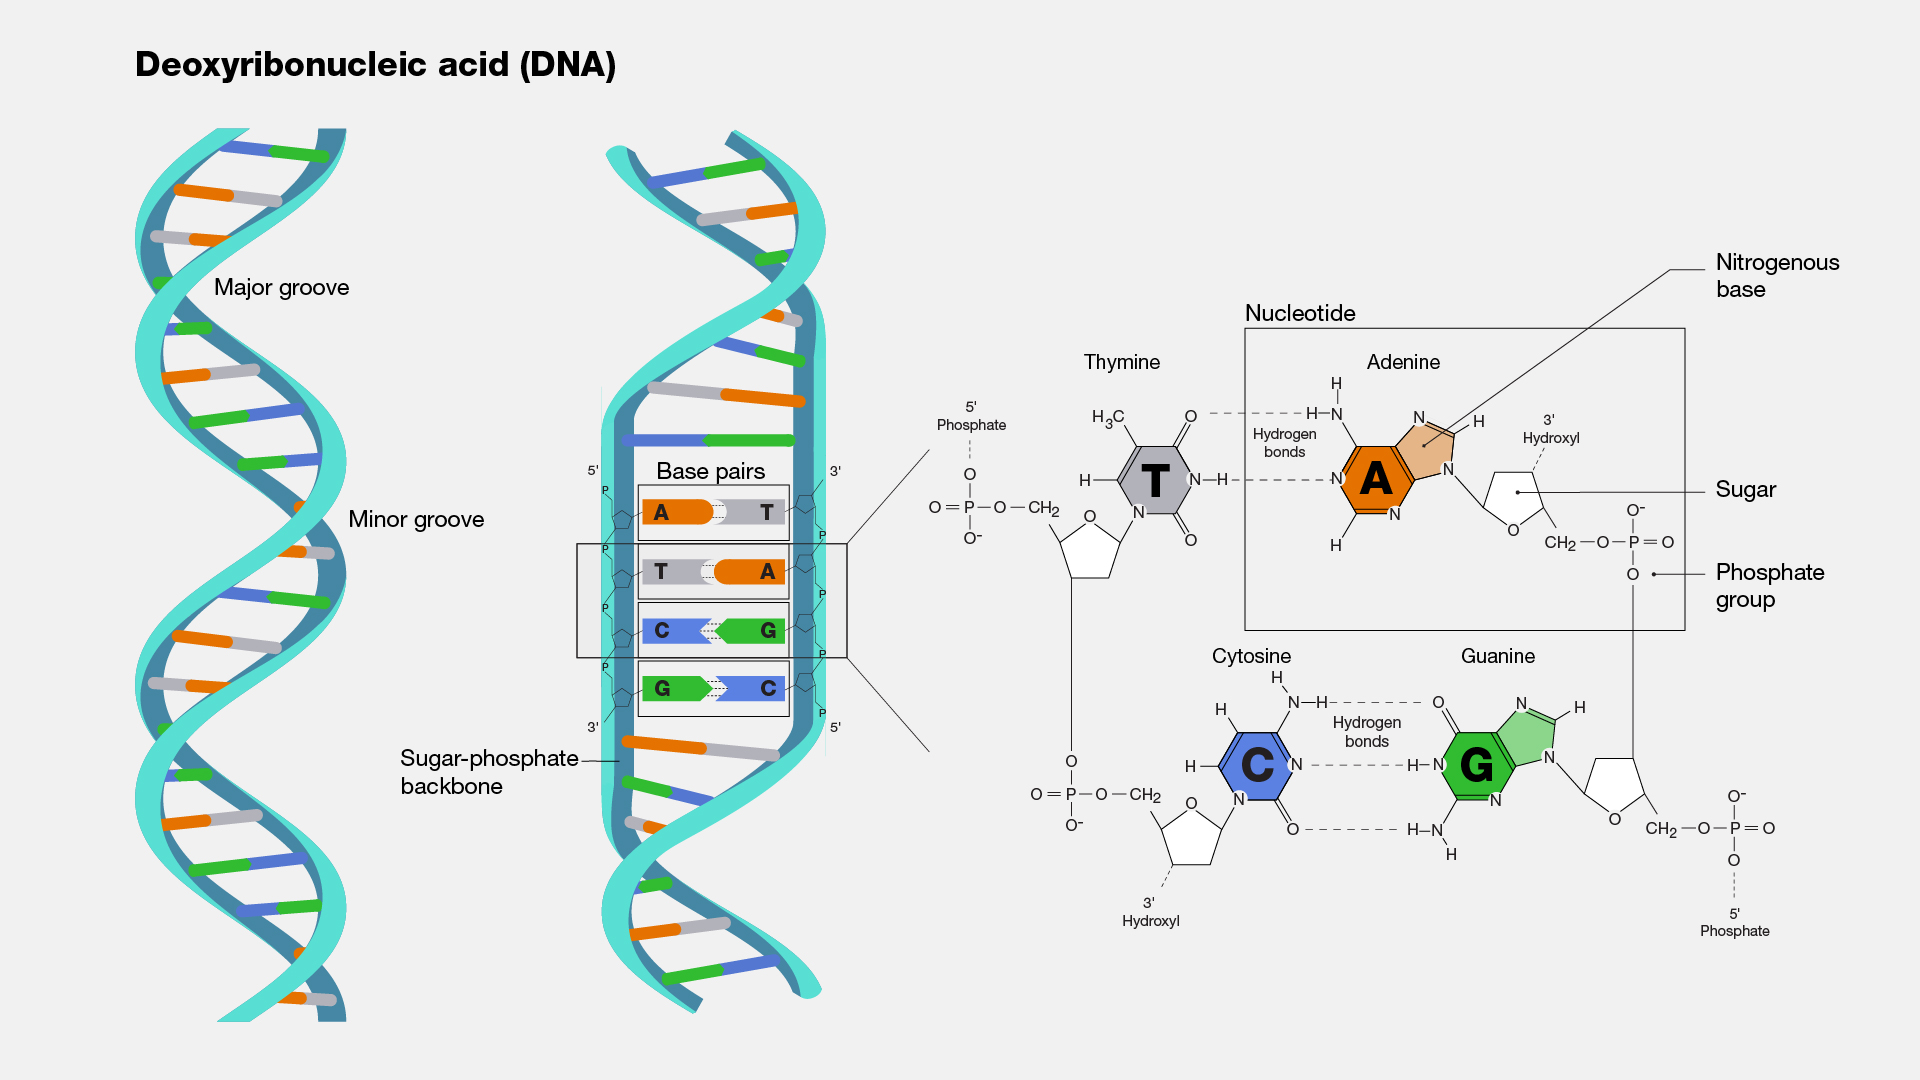
\includegraphics[width=0.95\textwidth]{figures/background/DNA_2024a.jpg}
		\caption[The DNA molecule]{The DNA molecule and the structure of the nucleotides, the basic piece of information of the DNA.} 
	\end{subfigure}%
	\\
	\begin{subfigure}[b]{0.75\textwidth}
		\centering
		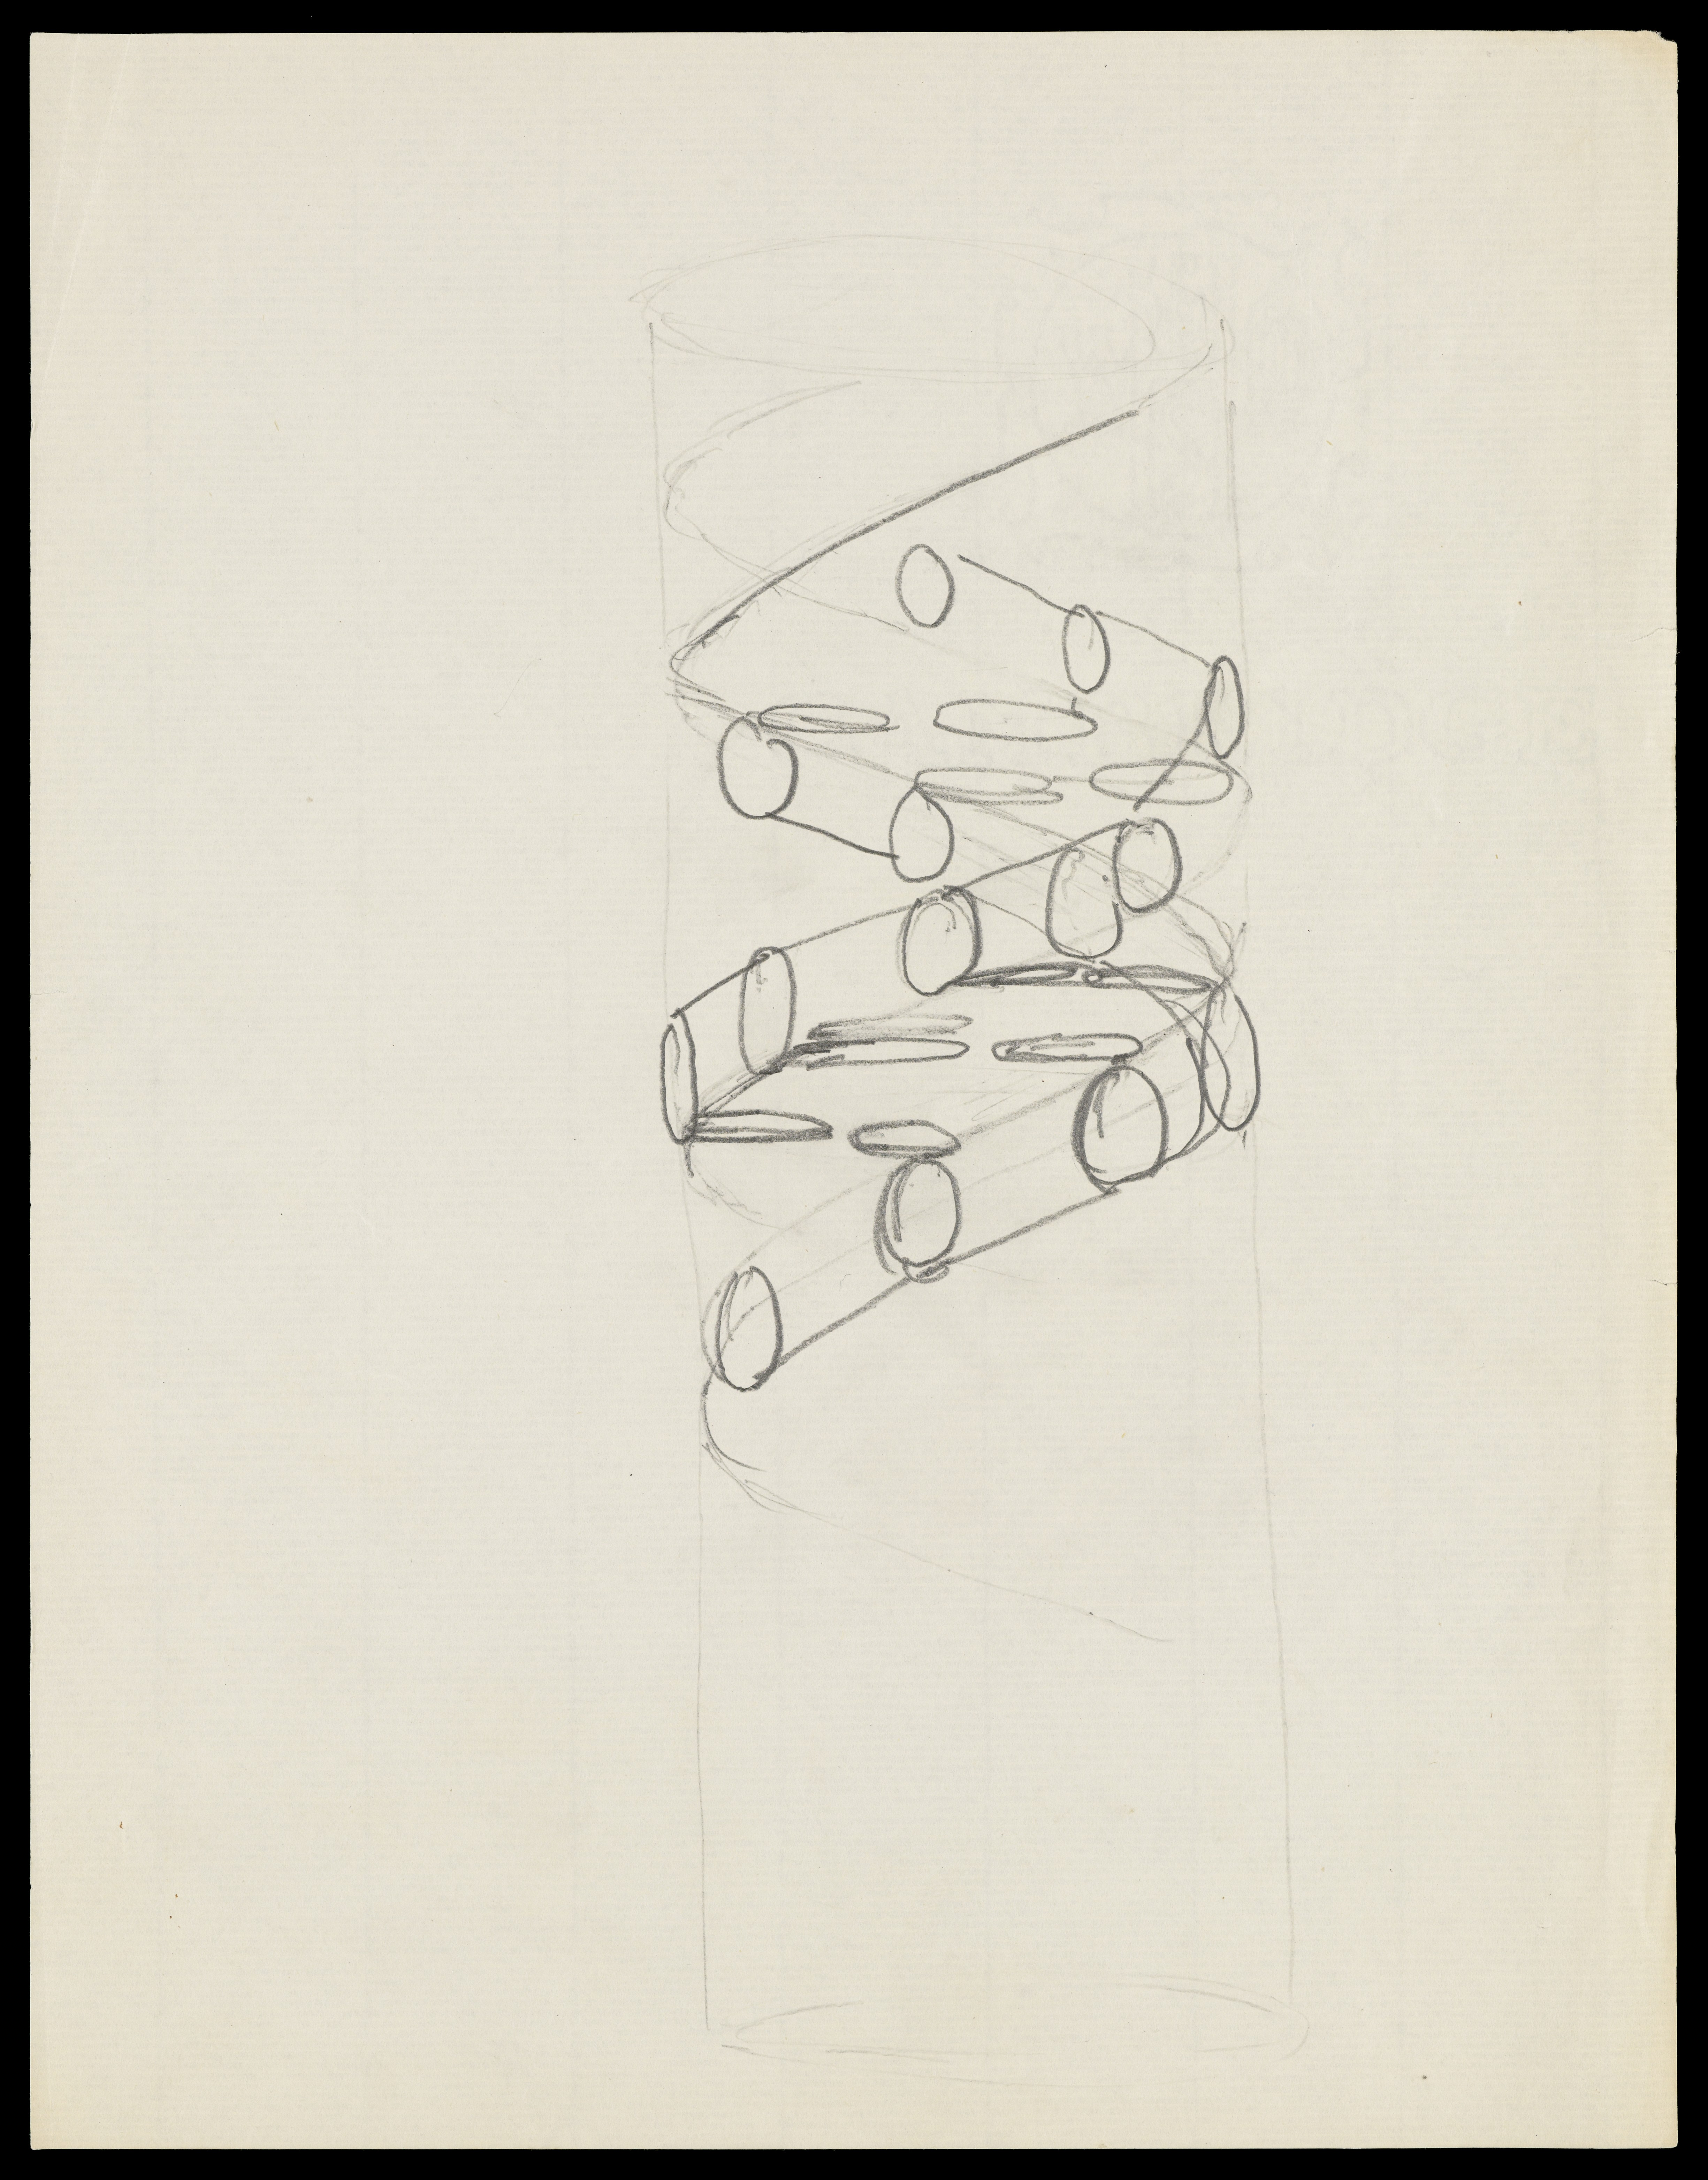
\includegraphics[width=0.95\textwidth]{figures/background/DNA_sketch.jpg}
		\caption[The DNA sketch by Crick]{The DNA molecule model draw by Francis Crick in 1953.} 
	\end{subfigure}%
\label{fig:DNA}
\end{figure}

\subsection{Next-generation and third generation sequencing}
In many biological disciplines, studying an organism's genetic information contained in its DNA is crucial. Over the years, researchers have developed various methods and techniques to extract this information from the cell nucleus. These processes typically involve two (or more) main steps. Here I describe the two main ones:
_{\begin{itemize}
	\item[DNA Extraction, Purification and Library preparation] The first step requires nontrivial biological manipulation of samples to extract DNA from cell nucleus and purify it without causing damage. This process isolates the genetic material from other cellular components, like RNA and proteins. The DNA molecule are fragmented into pieces of different length followed by 5′and 3′adapter ligation. 
	\item[DNA Sequencing] Next, specialized machines detect the sequence of nucleotides that compose the extracted DNA pieces. These techniques, called sequencing, use various, most of the time proprietary, technologies to determine the precise order of nucleotides (A, C, G, and T) in a DNA molecule. The raw data output of these machines are sequences of characters that are referred to as sequencing reads or simply reads.
\end{itemize}}
The landscape of DNA sequencing has evolved significantly since its inception. In 1977, Frederick Sanger and his colleagues introduced the first widely adopted sequencing method, known as chain termination sequencing or Sanger sequencing\cite{sanger_sequencing}. This innovative technique allowed scientists to read the sequence of nucleotides in a DNA molecule for the first time in a reliable and reproducible manner.
While Sanger sequencing has revolutionized genetic research, it has largely been replaced by more advanced technologies. These newer methods fall into two main categories:
Next Generation Sequencing (NGS) and Third Generation Sequencing. These technologies provide significant improvements in terms of speed, cost-effectiveness and data output compared to Sanger sequencing. \\
\textbf{Next Generation Sequencing} derives its name by launching a so-called next generation by revolutionizing sequencing with massive parallelization. This technology has continously improved since 2005 to yield up to 8 Terabases per single sequencing run, taking it maximum 2 days and dropping the price of, for example, a single individual sequenced per almost 100 dollars.
The output of these machines are reads of a length that varies between 150 and 300 bases and take the names of short reads. \\
One of the advances of the Next Generation sequencing is also the pair-end sequences, i.e. 


\section{Reads, \kmers and how to store them}

\section{Pangenomics, pangenomes and pangenome graphs}
\label{sec:background:pangenomics}
\subsection{The premisis for human pangenomics}
\large{\textbf{A LINEAR REFERENCE FOR ALL GENOMIC ANALYSES}}\\
Since the beginning of genomics, all analysis based on sequencing data depended upon the use of a single linear reference genome, i.e. the best assembled genome available for a species, to extract useful information from the DNA. We now know that this approach is suboptimal in a wide range of applications as a lot of genetic material of the species cannot be present in a single linear refererence: this is valid for eukariotes and even more for bacteria.  
\huge{\textbf{A SEQUENCING REVOLUTION}}\\
Right now we are witnessing a real revolution in the sequencing. As the price is significantly lowering, also thanks to competition of new companies entering the market, new scientific discoveries and technological advances are leading to a remarkable increase of quality, in term of per-base error rate, and throughput. This means than right now we dispose of a rich wealth of high quality sequencing information to produce hundreds or thousands of new first grade assemblies.

\huge{\textbf{A QUALITY REVOLUTION}}
This limitation at the beginning was not solvable due to the scarcity of high quality assembled genomes as the technologies of sequencing and computational tools were not mature enough. For example, the Human Genome Project took 13 years to produce its result~\cite{humangenomeproject} and the absence of long reads with decent error rate made it impossible to automatically resolve repetitive regions like telomers and centromeres~\cite{human-pangenomics-era}, producing a reference only $92\%$ complete~\cite{t2t}. This problem was only solved in 2022~\cite{t2t}. At the same time, many consortia are producing increasingly more genomes to a level comparable to the T2T consortium. For example, the HPRC, i.e. the Human Pangenome Reference Consortium released 47 new human genomes (92 haplotypes) in 2021 and has recently released other 153 genomes to a total of 400 haplotypes. The ability to produce such high quality data for human genomes is the main driver of the \\
Right now we are witnessing a real revolution in the sequencing. As the price is significantly lowering, also thanks to competition of new companies entering the market, new scientific discoveries and technological advances are leading to a remarkable increase of quality, in term of per-base error rate, and throughput. This means than right now we dispose of a rich wealth of high quality sequencing information to produce hundreds or thousands of new first grade assemblies.
This progress lead to a shift in paradigm with increasing effort from the scientific community to propose new methods to analyse one or multiple genomes: not anymore by comparing it against a single reference sequence but against a comprehensive representation of the species. \\
This novel way to overcome the limits of "linear genomic" and consider all the variation in a single species is called pangenomics. \\
Various efforts are being made on producing reference pangenomes of yeasts, bacterias, plants and animals, including humans. In order to do so, new tools to construct and then analyse and use such representations are being developed. 
It is important here to notice, as it will be stressed in the next sections and chapters, that construction is just the first step and that is very important to understand and work on which are the operations that can be succesfully performed by these representations. \\

\section{Graphs}

\subsection{De Bruijn Graphs}
\subsubsection{Colored and Compacted De Bruijn Graphs}
\subsection{Variation Graphs}

